\documentclass[11pt,a4paper]{article}
\usepackage[T1]{fontenc}
\usepackage{lmodern}
\usepackage{textcomp}
\usepackage[margin=2.2cm]{geometry}
\usepackage{microtype}
\usepackage{amsmath,amssymb}
\usepackage{graphicx}
\usepackage{booktabs,tabularx,array}
\usepackage{adjustbox}
\usepackage{float}
\usepackage{placeins}
\usepackage[numbers,sort&compress]{natbib}
\usepackage{xcolor}
\usepackage[colorlinks=true,linkcolor=blue!50!black,citecolor=blue!50!black,urlcolor=blue!50!black]{hyperref}
\usepackage{caption}
\captionsetup{font=small,labelfont=bf}
\setlength{\parskip}{3pt}
\newcommand{\FR}{FR@3}
\newcommand{\ET}{E[$T$]}
\newcommand{\labels}{\texttt{[LOCAL EXPLORATORY PILOT] [NOT PREREGISTERED] [NOT FOR CITATION] [DISCLOSE-BEFORE-USE]}}

\title{Twelve Bytes Against an Inverted Index:\\ What a Compact-Code Memory Retrieval Programme Found, and Which Configuration Choices Decided It}
\author{llmzip programme record, compiled by the programme's head researcher\\ \small \url{https://github.com/haliltalhaertan/llmzip-paper}}
\date{23 September 2026}

\begin{document}
\maketitle
\begin{center}\small\labels\end{center}

\begin{abstract}
\noindent
This report collects every result of a local research programme that asked whether a per-document 12-byte (96-bit) code, built from TF-IDF features projected by SVD and binarised, can replace or complement a BM25 index when an agent retrieves evidence from its conversational memory. Four benchmarks were used: LongMemEval-S, LoCoMo, PerLTQA and RealTalk. The programme was not preregistered and has no independent auditor. Its main transferable finding is methodological: five configuration choices each reversed a verdict while everything else was held fixed. These were the document unit, the query cohort, the projection family, the benchmark and the metric. On the product question the answer is negative. No compact budget reached BM25 on the pre-specified RealTalk gate; the best 48-byte cell was «c1.k384/qscale.BM25_coarse.fr3|2|s» «ci:c1.k384/qscale.BM25_coarse.fr3» pp on \FR{}. On LoCoMo the 96-bit code opens «reach.sign96.E_T» documents before the first piece of evidence (\ET{}), against «reach.bm25.E_T» for BM25 and a floor of «reach.floor» that the code's bits would allow. Engineering work produced two compactions that change no output bit. The encoder vocabulary shrank by «vocab.perltqa.saving_pct|1»--«vocab.locomo.saving_pct|1»\% and the BM25 index by «cbm25.LongMemEval.saving_pct|1»--«cbm25.LoCoMo.saving_pct|1»\%. Even after both, the encoder still needs «ratio.LoCoMo.compact»--«ratio.LongMemEval.compact» times the memory of the compacted BM25. Weighted rank fusion of BM25 with the code failed its pre-specified gate. A fixed fusion weight chosen after the fact lowers \ET{} on all four benchmarks without lowering \FR{}; it remains an unconfirmed lead. The report also lists the programme's «sup.entries|0» supersession entries and eleven errors made and corrected by its head researcher.
\end{abstract}

\section{Introduction}
Agents that keep long conversational histories must find the few turns relevant to a question among hundreds. The standard tool is a lexical inverted index scored by BM25~\citep{robertson2009bm25}. Its cost grows with the vocabulary. A tempting alternative is a fixed-size code per document, a few bytes of sign bits in the tradition of similarity hashing~\citep{charikar2002simhash,datar2004lsh} and learned binary codes~\citep{gong2013itq,jegou2011pq,ge2014opq,gao2024rabitq}. Such a code might route a query to its evidence at a small fraction of an index's footprint. The llmzip programme tested that idea on four public long-memory benchmarks~\citep{wu2024longmemeval,maharana2024locomo,du2024perltqa,lee2025realtalk}.

The programme did not find a code that beats BM25. It did find something of more general use, and that is the paper's first subject. Several of its intermediate verdicts turned on configuration choices that are rarely reported: how archive text is cut into documents, which queries are averaged, which projection family an ablation uses, which benchmark is measured and which metric decides. The literature on weak baselines and non-additive improvements~\citep{armstrong2009improvements,lin2019neuralhype} anticipates the general lesson. This record adds five concrete, fully measured instances from one programme.

The paper is written so that every result is visible from the document alone. Every number in the text, tables and figures is generated from a claims ledger of «meta:ledger_count» entries drawn from «meta:source_count» sources, each traced to a saved artefact with its SHA-256. Section~\ref{sec:setting} describes data and methods. Section~\ref{sec:results} gives the results. Section~\ref{sec:external} reviews two external strands. Section~\ref{sec:limits} discloses the process, including the errors.

\section{Setting, data and methods}\label{sec:setting}
\subsection{Benchmarks and data policy}
Table~\ref{tab:benchmarks} lists the four benchmarks. Each archive is one user's conversation history, and retrieval is always within one archive. LongMemEval-S has one question per archive, so its archive-clustered intervals reduce to an unclustered bootstrap over «cbm25.LongMemEval.queries_compared|0» single-query points. RealTalk carries no published licence. It was used locally only, and its data in the repository history is an open publication blocker that the repository owner must resolve.

\begin{table}[tbp]
\centering
\small
\caption{Benchmarks. Query counts are those scored by the bit-exactness checks and the fusion runs.}
\label{tab:benchmarks}
\begin{tabularx}{\linewidth}{@{}l r r l l >{\raggedright\arraybackslash}X@{}}
\toprule
Benchmark & Archives & Queries & Document unit & Licence & Scope \\
\midrule
LongMemEval-S (cleaned) & 470 & 470 & turn & MIT & 470 answerable questions; 30 abstention items excluded \\
LoCoMo & 10 & 1{,}535 & turn (dialogue line) & CC BY-NC 4.0 & category 5 excluded; five unscorable items dropped \\
PerLTQA & 30 & 8{,}265 & memory record & CC BY-NC 4.0 & all questions \\
RealTalk & 10 & 705 & message & none published & local use only; redistribution blocked \\
\bottomrule
\end{tabularx}
\end{table}


\subsection{Retrieval arms}
Each archive is fitted separately. The \emph{encoder} combines three channels: a word TF-IDF vectorizer (1--2 grams), a character TF-IDF vectorizer (\texttt{char\_wb}, 3--5 grams) and an LSA component. The concatenated representation is projected by a truncated SVD to $k\in\{96,192,384\}$ dimensions or left unprojected (\texttt{NOPROJ}). Documents are stored as $k$ sign bits, so 96 dimensions give 12 bytes per document. Query scoring differs by arm. In \texttt{sym} both sides are binarised. In \texttt{qscale} a scaled float query is scored against binary documents. In \texttt{float} both sides stay real-valued. \texttt{std} and \texttt{raw} denote the float arms with and without per-dimension standardisation. BM25 uses the textbook parameters $k_1=1.2$, $b=0.75$ over the same documents. Two BM25 analysers appear: a coarse one and the production (``frozen'') analyser, which is the stronger comparator.

\subsection{Metrics}
\FR{} is the expected fraction of a query's $m$ gold documents that appear among the first three results. It is computed in closed form over uniform random shuffling of tied scores, with no Monte-Carlo step. Hit@10 is the probability that at least one gold document appears in the first ten. \ET{} is the expected number of documents opened in the retriever's rank order until the first gold document; lower is better. It is the one metric on which a retriever can be compared with the memory-search lower bound $\mathrm{E}[T]\ge N/(2K)+1/2$, where $K=\min(2^{b},N)$ for $b$ routing bits and $N$ documents. The external review that supplied this bound is described in Section~\ref{sec:codex}. For multi-evidence questions we also report all@5, the fraction of queries whose gold documents all appear in the top five.

\subsection{Inference and gates}
All contrasts are paired by query. Intervals come from an archive-clustered bootstrap~\citep{efron1979bootstrap}: archives are resampled with replacement and the paired differences of their queries are pooled. The main analyses use «gate.fusion.reps|0|t» replicates with fixed seeds recorded in each run file. Where two arms were tested against one gate, intervals were widened to «gate.fusion.ci|1»\% (Bonferroni). Hyperparameters were chosen by leave-one-archive-out: the value minimising the objective on the other archives is applied to the held-out one. Every grid contains a no-op value that reproduces the baseline exactly.

A \emph{gate} is a decision rule written into the run record before the numbers were seen. Table~\ref{tab:gates} lists every gate in the programme. The house wording for an interval that contains zero is ``no significant difference was demonstrated''. It is never ``neutral'' or ``equivalent'', because no equivalence margin was declared in advance.

\begin{table}[tbp]
\centering
\small
\caption{Registry of pre-specified gates. "Min.\ effect" records whether the gate named a minimum useful effect size, not only significance.}
\label{tab:gates}
\begin{tabularx}{\linewidth}{@{}>{\raggedright\arraybackslash}p{3.3cm} >{\raggedright\arraybackslash}X l l >{\raggedright\arraybackslash}p{4.4cm}@{}}
\toprule
Gate & Criterion (declared before the run) & Min.\ effect & Outcome & Decisive numbers \\
\midrule
C3: code first stage, BM25 rerank (2026-09-16) & $\Delta$FR@3 $\geq 1.0$ pp over BM25, CI excluding 0 & yes & not met & LME \textminus{}0.33, PerLTQA +0.33, LoCoMo +1.07 pp (point estimates) \\
C1: compact code vs BM25, RealTalk (2026-09-20) & some arm $\leq$ 48 B/doc with $\Delta$FR@3 $\geq 2.0$ pp and 95\% CI excluding 0 & yes & fail & 0 of 12 cells positive; best \textminus{}1.11 [\textminus{}2.26, 0.05] pp \\
Channel ablation (2026-09-21) & drop the character channel only if no benchmark shows a significant FR@3 regression & no & fail & LME \textminus{}3.84, RealTalk \textminus{}2.69 pp, both significant \\
Vocabulary compaction (2026-09-21) & 0 differing bits, fewer bytes, latency $\leq 1.25\times$ & exactness & pass & 0 of 20{,}540 vectors differ; bytes \textminus{}63.6\% (LoCoMo) \\
Policy-shaped routing (2026-09-22) & E[T] significantly lower than static code ranking & no & pass (defective) & \textminus{}1.16 [\textminus{}2.22, \textminus{}0.15] docs; closes 9.7\% of the gap to BM25 \\
Fusion W, weighted RRF (2026-09-23) & LoCoMo E[T] cut $\geq 5$\% with 97.5\% CI below 0; FR@3 lower bound $>$ \textminus{}1.0 pp on all four & yes & fail & E[T] \textminus{}11.0\%; LoCoMo FR@3 \textminus{}3.90 [\textminus{}6.87, \textminus{}0.83] pp \\
Fusion G, gated switch (2026-09-23) & same as W & yes & fail & E[T] \textminus{}0.30 [\textminus{}1.52, 0.77] docs: no significant difference was demonstrated \\
\bottomrule
\end{tabularx}
\par\smallskip\parbox{\linewidth}{\footnotesize Gates were written into run records before results, but none was hash-committed in advance; see Section~\ref{sec:limits}.}
\end{table}


\subsection{Reproducibility harness}
A third independent environment (CPython 3.14.7, NumPy 2.5.3, SciPy 1.18.1, scikit-learn 1.9.1 on native Windows) reproduced all «t1.cells_match|0» of «t1.cells|0» published RealTalk cells. Of «t1.evaluations|0» evaluations, «t1.exact|0» were exact. The remaining «t1.deviating|0» came from one query that flips at the rank-3 boundary under hash-seed-dependent iteration order. That flip moves one BM25 cell between «t1.bistable_published|4» and «t1.bistable_alt|4», a difference of «t1.bistable_diff|4» pp. Sorting the iteration fixes it. The sealed snapshot's manifest of «seal.entries|0» entries was reissued with «seal.changed|0» changed files and no changed number.

\section{Results}\label{sec:results}
\subsection{Five configuration choices each reversed a verdict}\label{sec:reversals}
Table~\ref{tab:reversals} and Figure~\ref{fig:reversals} hold one choice fixed at a time.

\emph{Document unit.} The external package that prompted the LoCoMo audit reported BM25 \FR{} «locomo_gap.external_reported» on «locomo_gap.external_n|0|t» queries. This project measured «locomo_gap.mean.A_project» on «cbm25.LoCoMo.queries_compared|0|t» queries, a gap of «locomo_gap.total_gap_from_project» pp. Rebuilding the arms one change at a time located the whole gap in how dialogue text is cut into documents. The document unit alone accounts for «locomo_gap.document_unit» pp, leaving a residual of «locomo_gap.residual_after_document_unit|3» pp (Figure~\ref{fig:reversals}a). Removing the image captions that the project appended to «locomo_gap.captions_docs|0|t» documents moves BM25 by «locomo_gap.image_captions_alone|2|s» pp; adding session timestamps moves it by «locomo_gap.timestamps_alone|2|s» pp. The unit also changes significance. The full raw float arm trails BM25 by «n2.project.all.raw_full-bm25|2|s» «ci:n2.project.all.raw_full-bm25» pp under the project unit. Under the external unit the difference is «n2.external.all.raw_full-bm25|2|s» «ci:n2.external.all.raw_full-bm25» pp, and no significant difference was demonstrated.

\emph{Cohort.} The five contrasts in the sealed LoCoMo audit had been computed on a rare-term bucket of «n2.project.n_rare|0» queries. They were later quoted as LoCoMo-wide results. Re-running them on all «n2.project.n|0|t» queries left every direction unchanged but moved magnitudes and significance. The 48-byte minus 12-byte sign contrast falls from «n2.project.rare.sym_384-sym_96|2|s» to «n2.project.all.sym_384-sym_96|2|s» pp. The full-dimension sign arm's deficit against BM25 is significant in the rare bucket, «n2.project.rare.sym_full-bm25|2|s» «ci:n2.project.rare.sym_full-bm25», but not on all queries, «n2.project.all.sym_full-bm25|2|s» «ci:n2.project.all.sym_full-bm25». The comparison that mattered for the product claim, 48-byte sign against BM25, is non-significant in all four unit $\times$ cohort cells, and its sign follows the document unit, not the cohort: «n2.project.rare.sym_384-bm25|2|s», «n2.project.all.sym_384-bm25|2|s», «n2.external.rare.sym_384-bm25|2|s» and «n2.external.all.sym_384-bm25|2|s» pp (Figure~\ref{fig:reversals}b; all cells in Table~\ref{tab:n2}).

\emph{Projection family.} Among unprojected float arms on RealTalk, dropping the character and LSA channels \emph{helped}: \FR{} «ladder.diff.NOPROJ_WORD/float-vs-NOPROJ_FULL/float.fr3|2|s» «ci:ladder.diff.NOPROJ_WORD/float-vs-NOPROJ_FULL/float.fr3» pp and Hit@10 «ladder.diff.NOPROJ_WORD/float-vs-NOPROJ_FULL/float.hit10|2|s» «ci:ladder.diff.NOPROJ_WORD/float-vs-NOPROJ_FULL/float.hit10» pp. In the production configuration ($k=96$, sign codes) the same comparison on the same benchmark \emph{hurt}: «chan.RealTalk.WORD.d|2|s» «ci:chan.RealTalk.WORD» pp (Figure~\ref{fig:reversals}c). A lead from the first family would have been a false memory saving in the second.

\emph{Benchmark.} The pre-specified channel ablation removed the character channel at $k=96$. \FR{} changed by «chan.LME.WORD.d|2|s» «ci:chan.LME.WORD» pp on LongMemEval, «chan.RealTalk.WORD.d|2|s» on RealTalk and «chan.LoCoMo.WORD.d|2|s» «ci:chan.LoCoMo.WORD» on LoCoMo, where no significant difference was demonstrated. On PerLTQA it changed by «chan.PerLTQA.WORD.d|2|s» «ci:chan.PerLTQA.WORD» (Figure~\ref{fig:reversals}d; Table~\ref{tab:channels}). Had only PerLTQA been measured, the channel would have been dropped for a «expr:100*(1-{chan.PerLTQA.WORD.mb}/{chan.PerLTQA.LSA_WORD_CHAR.mb})|0»\% memory saving, and two benchmarks would have been damaged without anyone noticing. The gate failed and the channel stays.

\emph{Metric.} The weighted-fusion arm of Section~\ref{sec:fusion} lowers LoCoMo \ET{} by «fusion.LoCoMo.W.dE_T|2|a» «ci:fusion.LoCoMo.W.dE_T|2|a» documents, a significant improvement. It lowers \FR{} by «fusion.LoCoMo.W.dFR3|2|a» «ci:fusion.LoCoMo.W.dFR3|2|a» pp, a significant loss (Figure~\ref{fig:reversals}e). Whether the arm is better depends entirely on which metric is declared primary.

A sixth candidate, the tie convention, is listed in Table~\ref{tab:reversals} for completeness. Reporting deterministic ties (fr3) instead of their expectation (efr3) moves the external BM25 value by «locomo_gap.arm_E_minus_reported|2|s» pp but reverses no verdict. Earlier summaries in the programme counted it among the reversals; that was an overstatement.

\begin{figure}[t]
\centering
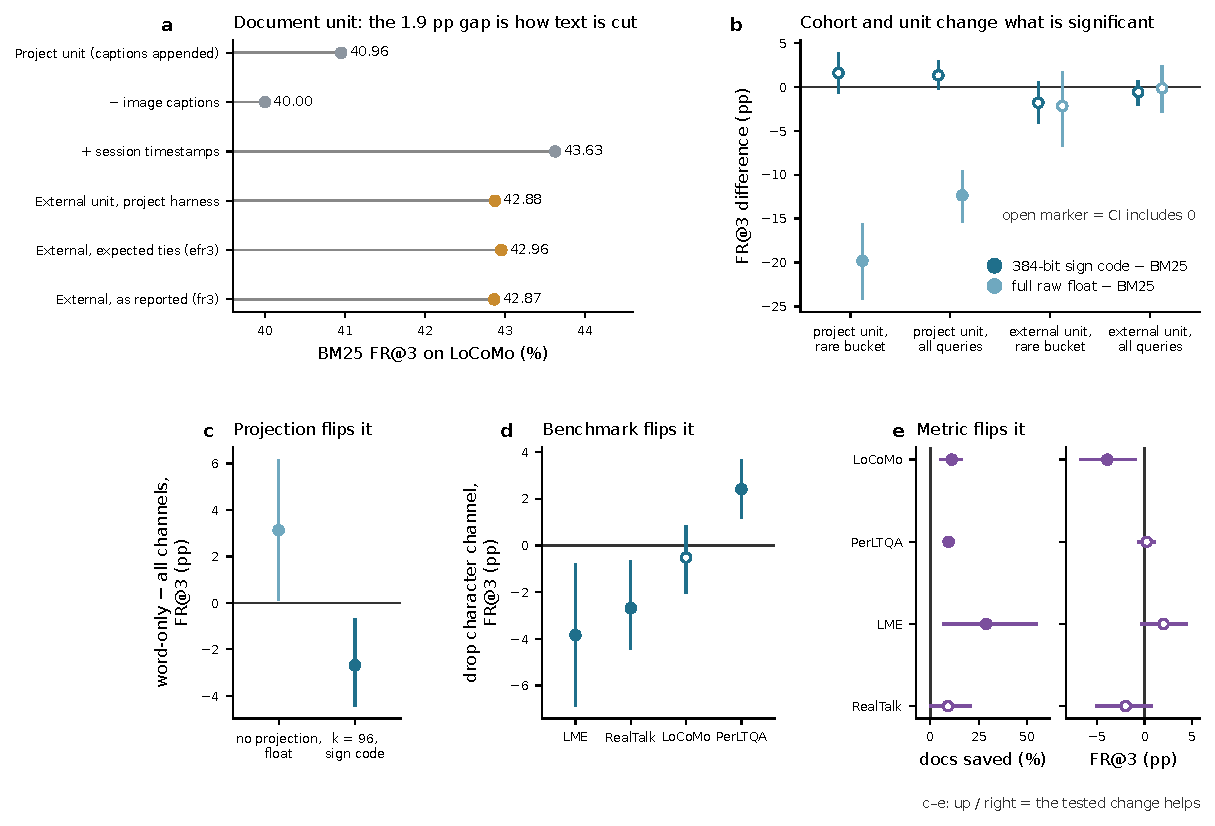
\includegraphics[width=\linewidth]{figures/fig1_reversals.pdf}
\caption{Five configuration choices, each changed with everything else fixed. (a)~BM25 \FR{} on LoCoMo as the document unit is rebuilt step by step. (b)~LoCoMo contrasts in the four unit $\times$ cohort cells; open markers: the interval includes 0. (c)~Word-only minus all channels on RealTalk, unprojected float against the $k=96$ sign code. (d)~Removing the character channel on four benchmarks (LME = LongMemEval). (e)~Weighted fusion W against BM25: documents saved and \FR{} change. Intervals 95\%, except (e) 97.5\%.}
\label{fig:reversals}
\end{figure}

\begin{table}[tbp]
\centering
\footnotesize
\caption{One configuration choice at a time, everything else held fixed. FR@3 differences in pp unless stated. Intervals are 95\% paired, archive-clustered bootstraps except the metric row (97.5\%). $^{\circ}$ interval includes 0: no significant difference was demonstrated.}
\label{tab:reversals}
\begin{adjustbox}{max width=\linewidth}\begin{tabular}{@{}l >{\raggedright\arraybackslash}p{3.4cm} >{\raggedright\arraybackslash}p{2.2cm} l >{\raggedright\arraybackslash}p{2.2cm} l@{}}
\toprule
Choice & Quantity & Setting A & Value A & Setting B & Value B \\
\midrule
Document unit & full raw float $-$ BM25, all queries & project unit & \textminus{}12.36 [\textminus{}15.47, \textminus{}9.50] & external unit & \textminus{}0.17 [\textminus{}2.90, 2.45]$^{\circ}$ \\
Cohort & full sign code $-$ BM25, project unit & rare bucket & \textminus{}3.77 [\textminus{}6.51, \textminus{}0.63] & all queries & \textminus{}1.75 [\textminus{}3.61, 0.68]$^{\circ}$ \\
Projection family & word-only $-$ all channels, RealTalk & no projection, float & +3.12 [0.08, 6.17] & $k=96$ sign code & \textminus{}2.69 [\textminus{}4.45, \textminus{}0.66] \\
Benchmark & drop character channel & PerLTQA & +2.40 [1.14, 3.67] & LongMemEval & \textminus{}3.84 [\textminus{}6.88, \textminus{}0.75] \\
Metric & fusion W $-$ BM25, LoCoMo & E[T], docs (lower is better) & \textminus{}6.95 [\textminus{}10.60, \textminus{}2.94] & FR@3 & \textminus{}3.90 [\textminus{}6.87, \textminus{}0.83] \\
Tie convention$^{\dagger}$ & external BM25 FR@3, LoCoMo (\%) & deterministic (fr3) & 42.87 & expected over ties (efr3) & 42.96 (+0.09) \\
\bottomrule
\end{tabular}\end{adjustbox}
\par\smallskip\parbox{\linewidth}{\footnotesize $^{\dagger}$ Included for completeness: the tie convention moves the number but reverses no verdict in this programme.}
\end{table}


\subsection{The 12-byte code does not beat BM25}\label{sec:verdict}
\emph{Pre-specified gate.} C1 required some arm of at most 48 bytes per document to beat BM25 by at least «gate.c1.min_pp|1» pp \FR{} on RealTalk, with a «gate.c1.ci|0»\% interval excluding zero. Twelve cells were measured: six arms against the two BM25 analysers. None is positive (Figure~\ref{fig:verdict}a; Table~\ref{tab:c1}). At 12 bytes the code trails the coarse BM25 by «c1.k96/sym.BM25_coarse.fr3|2|s» «ci:c1.k96/sym.BM25_coarse.fr3» pp. The best cell, 48 bytes with query scaling, trails it by «c1.k384/qscale.BM25_coarse.fr3|2|s» «ci:c1.k384/qscale.BM25_coarse.fr3». Against the production analyser it trails by «c1.k384/qscale.BM25_frozen.fr3|2|s» «ci:c1.k384/qscale.BM25_frozen.fr3». The only cell ever presented as a win was a Hit@10 difference of «c1.k384/qscale.BM25_coarse.hit10|2|s» «ci:c1.k384/qscale.BM25_coarse.hit10» against the weaker analyser. Its interval contains zero.

\emph{An arm never reported before.} While assembling this paper we found one RealTalk ladder arm that had been computed but never reported: the unprojected, full-vocabulary representation with query scaling (\texttt{NOPROJ\_FULL/qscale}). Against the production BM25 it gains «ladder.diff.NOPROJ_FULL/qscale-vs-BM25_frozen/-.fr3|2|s» «ci:ladder.diff.NOPROJ_FULL/qscale-vs-BM25_frozen/-.fr3» pp \FR{}. For Hit@10 the difference is «ladder.diff.NOPROJ_FULL/qscale-vs-BM25_frozen/-.hit10|2|s» «ci:ladder.diff.NOPROJ_FULL/qscale-vs-BM25_frozen/-.hit10», and no significant difference was demonstrated. This arm is not compact, was found post hoc, was measured on one benchmark and was never gated. It is reported so that it is not lost, not as a finding (grey rows in Figure~\ref{fig:verdict}a; all seventeen ladder arms in Table~\ref{tab:ladder}).

\emph{Expected documents opened.} On LoCoMo (Figure~\ref{fig:verdict}b), scanning without an index opens «reach.no_index» documents on average. The 96-bit sign code opens «reach.sign96.E_T» (median «reach.sign96.median|0»). The same projection kept in float opens «reach.float96.E_T» (median «reach.float96.median|0»), and BM25 opens «reach.bm25.E_T» (median «reach.bm25.median|0»). The bound for 96 routing bits is «reach.floor». All three retrievers remove most of the scan and sit within a few tens of percent of each other, yet each is far above what its bits would allow. The byte budget is therefore not the binding constraint; the map from query to address is.

\emph{Earlier routes.} Two owner-proposed ideas had been run before this programme's audits (Figure~\ref{fig:verdict}c--d). Using the 96-bit code as a first stage and reranking its top 50 by BM25 over the original text changes \FR{} by «gate.c3.LME.delta|2|s», «gate.c3.PerLTQA.delta|2|s» and «gate.c3.LoCoMo.delta|2|s» pp on LongMemEval, PerLTQA and LoCoMo. That is below the C3 gate's «gate.c3.min_pp|1» pp on two of three. The same reranker over a float first stage does as well, so the gain belongs to the reranker. Replacing each archive's fitted vocabulary by a shared hashed encoder roughly halves \FR{}. On LongMemEval it falls from «hashed.LME.base192.fr3» to «hashed.LME.shared_seed2026091601.fr3»\%, on PerLTQA from «hashed.PerLTQA.base192.fr3» to «hashed.PerLTQA.shared_seed2026091601.fr3»\% and on LoCoMo from «hashed.LoCoMo.base192.fr3» to «hashed.LoCoMo.shared_seed2026091601.fr3»\%. The per-archive lexical statistics carry the quality.

\begin{figure}[t]
\centering
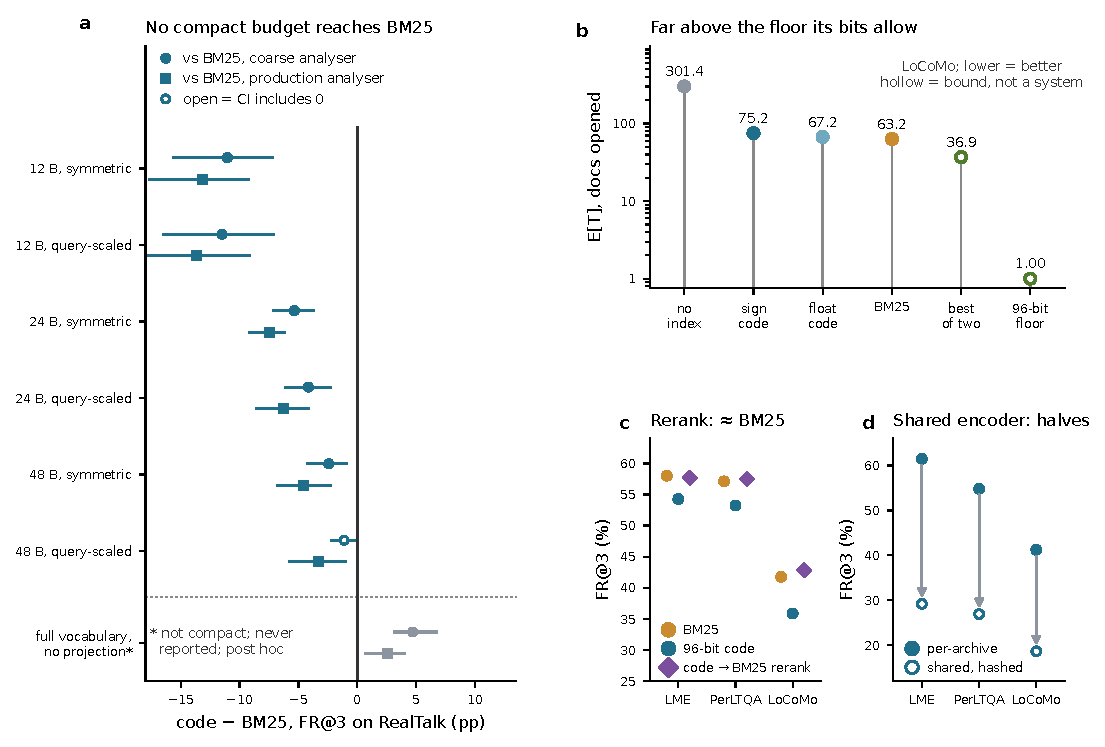
\includegraphics[width=\linewidth]{figures/fig2_compact_vs_bm25.pdf}
\caption{The compact code against BM25. (a)~C1 gate on RealTalk: code minus BM25 \FR{} for six arms and two BM25 analysers; open markers: the interval includes 0. Grey: the unprojected, full-vocabulary arm, which is not compact and was found post hoc. (b)~\ET{} on LoCoMo (log scale); hollow markers are bounds, not systems. (c)~Code first stage with BM25 reranking. (d)~Per-archive against shared hashed encoder.}
\label{fig:verdict}
\end{figure}

\subsection{Memory: the vocabulary is the cost, and it compacts losslessly}\label{sec:memory}
\emph{Where the bytes are.} A reachable-object walk from named serving roots over ten LoCoMo archives gives the following decomposition (Figure~\ref{fig:memory}a). The character vocabulary takes «resident.cv_char_vectorizer|2|m» MB and the word vocabulary «resident.wv_word_vectorizer|2|m» MB. The packed 96-bit document codes take «resident.packed_doc_codes|1|k» kB, «expr:100*{resident.packed_doc_codes}/{resident.union}|1»\% of the «resident.union|2|m» MB total, and the raw text «resident.raw_text|2|m» MB. The code is already negligible, so compressing it further cannot matter. The cost is the per-archive fitted encoder, and that same object carries the quality.

\emph{Bit-identical compaction.} Two structural rewrites keep every output bit (Table~\ref{tab:compaction}; Figure~\ref{fig:memory}b). First, the encoder's term dictionaries were replaced by a sorted UTF-8 blob with offsets and a fixed-width key array searched by binary search. This cut vocabulary bytes by «vocab.locomo.saving_pct|1»\% on LoCoMo, «vocab.perltqa.saving_pct|1»\% on PerLTQA and «vocab.lme.saving_pct|1»\% on LongMemEval. Over «expr:{vocab.locomo.vectors}+{vocab.perltqa.vectors}+{vocab.lme.vectors}|0|t» query vectors there were «expr:{vocab.locomo.mismatch}+{vocab.perltqa.mismatch}+{vocab.lme.mismatch}|0» differing bits, and latency ratios were «vocab.perltqa.latency|2»--«vocab.lme.latency|2». Second, BM25 was stored as a term-major compressed sparse row with a sorted vocabulary blob. This cut its bytes by «cbm25.LongMemEval.saving_pct|1»--«cbm25.LoCoMo.saving_pct|1»\%, with zero differing float64 scores over «expr:{cbm25.LoCoMo.queries_compared}+{cbm25.PerLTQA.queries_compared}+{cbm25.LongMemEval.queries_compared}+{cbm25.RealTalk.queries_compared}|0|t» queries. Because both changes are exact, quality was not re-measured and is claimed only as measured bit equality. Separately, the repository owner's F1--F4 chain on the encoder object graph went from «f1.before|0|t» to «f1.after|0|t», «f2.after|0|t» and finally «f4.after|0|t» bytes, «f1f4.total_saving_pct|2»\% less in total. The warm single-query median fell from «f4.ms_before|2» to «f4.ms_after|2» ms, also with bit-identical retrieval.

\emph{A fair comparison.} Earlier notes compared a compacted encoder with a stock dictionary BM25 and reported a ratio of about nine. Treating both sides equally changes the picture. The stock ratio of encoder to BM25 memory is «ratio.LoCoMo.stock», «ratio.PerLTQA.stock» and «ratio.LongMemEval.stock» on LoCoMo, PerLTQA and LongMemEval. With both sides compacted it is «ratio.LoCoMo.compact», «ratio.PerLTQA.compact» and «ratio.LongMemEval.compact» (Figure~\ref{fig:memory}c). Compaction helps BM25 more than the encoder. All byte counts are reachable-object accounting, not process RSS. The stock BM25 is a plain Python implementation, never compared with Lucene or similar engines. These savings make the existing system cheaper; they do not make it better.

\begin{figure}[t]
\centering
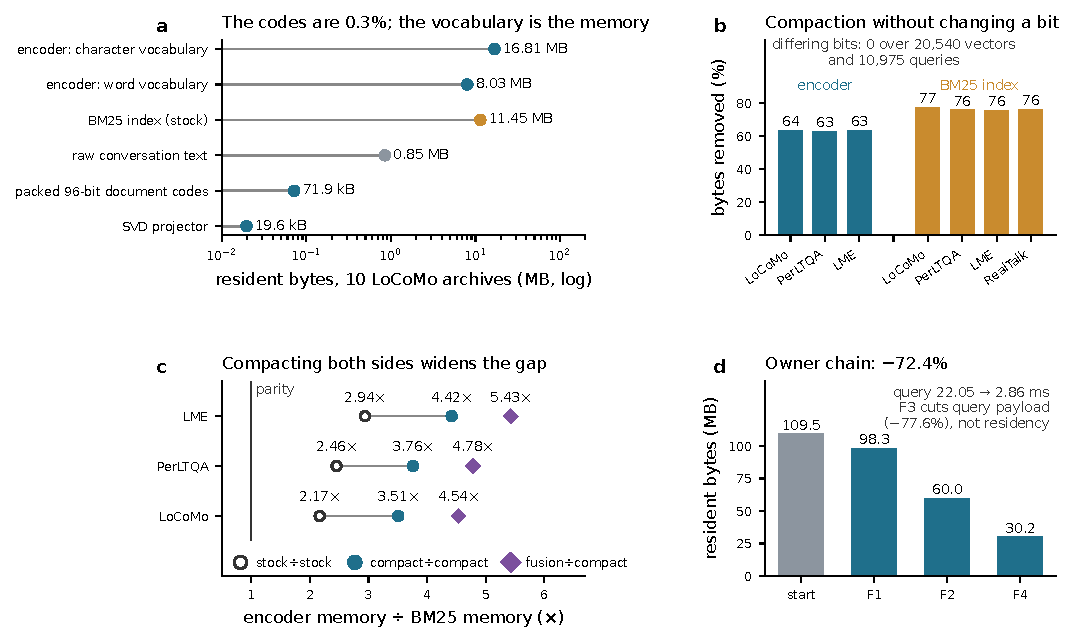
\includegraphics[width=\linewidth]{figures/fig3_memory.pdf}
\caption{Memory. (a)~Resident bytes over ten LoCoMo archives (log scale). (b)~Bytes removed by the two bit-identical compactions. (c)~Encoder memory over BM25 memory with both sides stock, both compacted, and for the fused system. (d)~The owner's F1--F4 chain on the encoder object graph.}
\label{fig:memory}
\end{figure}

\begin{table}[tbp]
\centering
\footnotesize
\caption{Bit-identical compaction. MB are summed over archives; "bits" counts differing outputs over all compared query vectors or query score lists; "time" is compact/stock latency. The last three columns compare resident bytes; "fusion" is BM25 + encoder + codes over compact BM25.}
\label{tab:compaction}
\begin{adjustbox}{max width=\linewidth}\begin{tabular}{@{}l r r r r r r r r r r r@{}}
\toprule
& \multicolumn{4}{c}{Encoder vocabulary} & \multicolumn{4}{c}{BM25 index} & \multicolumn{3}{c}{Encoder $\div$ BM25} \\
\cmidrule(lr){2-5}\cmidrule(lr){6-9}\cmidrule(l){10-12}
Benchmark & MB & $-$\% & bits & time & MB & $-$\% & bits & time & stock & compact & fusion \\
\midrule
LoCoMo & 24.8 $\to$ 9.1 & 63.6 & 0/3{,}070 & 0.93 & 11.45 $\to$ 2.58 & 77.5 & 0/1{,}535 & 0.22 & 2.17 & 3.51 & 4.54 \\
PerLTQA & 79.1 $\to$ 29.3 & 62.9 & 0/16{,}530 & 0.92 & 32.20 $\to$ 7.80 & 75.8 & 0/8{,}265 & 0.28 & 2.46 & 3.76 & 4.78 \\
LongMemEval & 5{,}244.9 $\to$ 1{,}915.4 & 63.5 & 0/940 & 0.95 & 1{,}783.08 $\to$ 433.36 & 75.7 & 0/470 & 0.21 & 2.94 & 4.42 & 5.43 \\
RealTalk & \multicolumn{4}{c}{not measured} & 13.70 $\to$ 3.25 & 76.3 & 0/705 & 0.14 & -- & -- & -- \\
\bottomrule
\end{tabular}\end{adjustbox}
\par\smallskip\parbox{\linewidth}{\footnotesize Owner chain F1--F4 on the encoder object graph: 109{,}515{,}058 $\to$ 30{,}175{,}450 B (72.45\% less); warm single-query median 22.05 $\to$ 2.86 ms. Byte counts are reachable-object accounting, not process RSS, and the stock BM25 is a plain Python dictionary implementation.}
\end{table}


\subsection{Expected cost, policy shaping and headroom}\label{sec:reach}
BM25's advantage on \ET{} is concentrated early: its median query opens «reach.bm25.median|0» documents against «reach.sign96.median|0» for the code (Figure~\ref{fig:cost}a). A policy-shaped variant penalises, after each non-gold document is opened, the remaining documents whose codes resemble it; it reads only the packed codes. It lowered the code's \ET{} from «policy.code.static» to «policy.code.adaptive», a change of «policy.code.delta|2|s» «ci:policy.code» documents, with the penalty weight $\lambda$ chosen out of fold. The same penalty applied to BM25 is rejected by leave-one-archive-out ($\lambda=0$ in every archive), so the gain comes from the code's document geometry and not from generic diversification (Figure~\ref{fig:cost}b). The arm passed its gate, but the gate named no minimum effect. The gain closes «policy.closed_bm25_pct|1»\% of the «policy.gap_to_bm25|2»-document gap to BM25 and «policy.closed_floor_pct|2»\% of the gap to the floor, which is too little to change any decision.

The two rankings are complementary (Figure~\ref{fig:cost}c). The code reaches the first gold document strictly earlier than BM25 on «reach.code_better_pct|1»\% of queries and ties on «reach.tie_pct|1»\%. A per-query oracle that always picks the better of the two would reach \ET{} «reach.oracle_min». Simple alternation of the two lists gives «reach.interleave», worse than BM25 alone. The oracle is an unattainable bound, but it shows that the code carries information BM25 lacks on about a third of queries.

\begin{figure}[t]
\centering
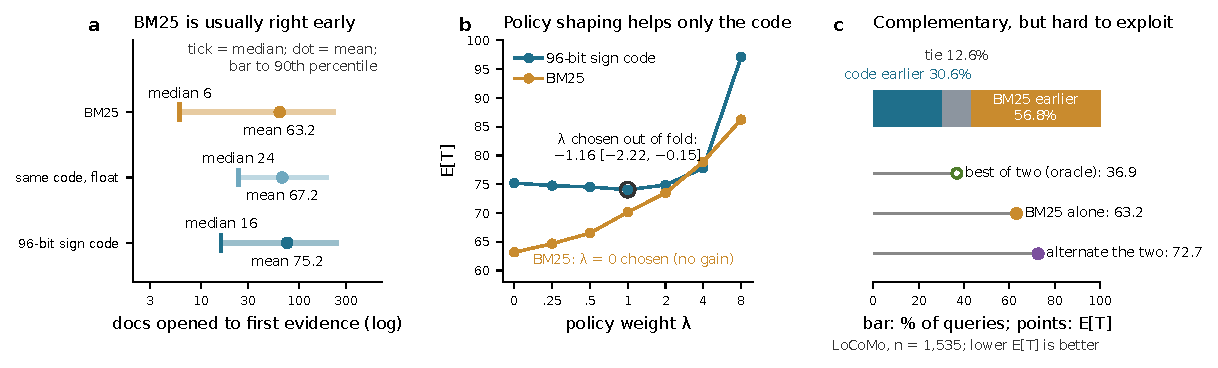
\includegraphics[width=\linewidth]{figures/fig4_expected_cost.pdf}
\caption{Expected cost on LoCoMo. (a)~Per-query documents opened: median (tick), mean (dot) and range to the 90th percentile. (b)~\ET{} of the policy-shaped penalty against its weight $\lambda$, for the code and for BM25. (c)~Share of queries on which each ranking reaches evidence first, and \ET{} of the oracle, BM25 and alternation.}
\label{fig:cost}
\end{figure}

\subsection{Fusion: the gate failed; a post-hoc lead remains}\label{sec:fusion}
An unweighted reciprocal-rank fusion~\citep{cormack2009rrf} of BM25 and the code had already lost on LoCoMo in an earlier configuration. There it changed \FR{} by «rrf16.locomo.fr3|2|s» «ci:rrf16.locomo.fr3» pp. The programme therefore tested two arms that can fall back to BM25 exactly. W is weighted RRF with score $1/(61+r_{\text{BM25}}) + w/(61+r_{\text{code}})$, with $w$ chosen out of fold. G is a gated switch on BM25's top score. The gate was written with a minimum effect. On LoCoMo, \ET{} had to fall by at least «gate.fusion.min_cut_pct|0»\% with a «gate.fusion.ci|1»\% interval below zero. On all four benchmarks, the lower bound of the \FR{} difference had to stay above «gate.fusion.margin_pp|1» pp.

Both arms failed (Table~\ref{tab:fusion}; Figure~\ref{fig:fusion}). W met the primary criterion, cutting LoCoMo \ET{} by «expr:-100*{fusion.LoCoMo.W.dE_T}/{fusion.LoCoMo.bm25.E_T}|1»\%. It failed non-inferiority on LoCoMo, «fusion.LoCoMo.W.dFR3|2|s» «ci:fusion.LoCoMo.W.dFR3», and on RealTalk, «fusion.RealTalk.W.dFR3|2|s» «ci:fusion.RealTalk.W.dFR3». For G, no significant difference was demonstrated anywhere.

After seeing the weight grid, a fixed $w=0.1$ lowered \ET{} significantly on all four benchmarks. On LoCoMo the reduction was «posthoc.LoCoMo.dE_T|2|a» «ci:posthoc.LoCoMo.dE_T|2|a» documents. \FR{} fell on none of the four, and all its lower bounds stay above «gate.fusion.margin_pp|1» pp. On the all-evidence measure it gains «allev.LoCoMo.w0.1.dall@5|2|s», «allev.PerLTQA.w0.1.dall@5|2|s», «allev.LongMemEval.w0.1.dall@5|2|s» and «allev.RealTalk.w0.1.dall@5|2|s» pp all@5 on LoCoMo, PerLTQA, LongMemEval and RealTalk. It still misses the primary threshold: the LoCoMo cut is «expr:-100*{posthoc.LoCoMo.dE_T}/{fusion.LoCoMo.bm25.E_T}|1»\% against «gate.fusion.min_cut_pct|0»\%. Because $w$ was chosen after the grid was seen and every on-disk benchmark has now been looked at, this is a lead that needs a hash-committed test on unseen data, not a finding. Fusion also has a price. The query must be encoded, so the fused system needs «ratio.LoCoMo.fused», «ratio.PerLTQA.fused» and «ratio.LongMemEval.fused» times the memory of compact BM25.

\begin{figure}[t]
\centering
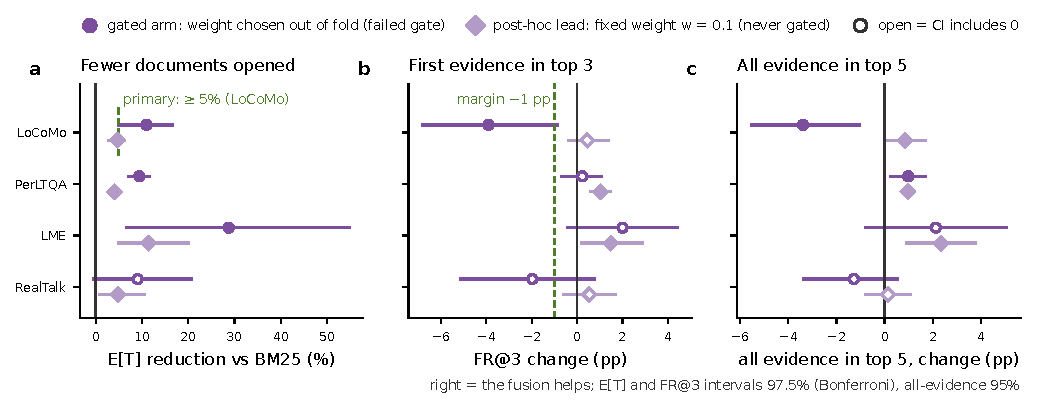
\includegraphics[width=\linewidth]{figures/fig5_fusion.pdf}
\caption{BM25 + code fusion against BM25. Filled circles: the gated arm with its weight chosen out of fold, which failed the gate. Diamonds: the fixed weight $w=0.1$ chosen after the grid was seen, never gated. Dashed lines: the gate's thresholds. Open markers: the interval includes 0.}
\label{fig:fusion}
\end{figure}

\begin{table}[tbp]
\centering
\footnotesize
\caption{Fusion of BM25 with the 96-bit code by weighted reciprocal rank. E[T] in documents opened (lower is better), FR@3 in pp. E[T] and FR@3 intervals are 97.5\% (Bonferroni over two arms); all-evidence intervals are 95\%.}
\label{tab:fusion}
\begin{adjustbox}{max width=\linewidth}\begin{tabular}{@{}l r l l l l r l@{}}
\toprule
& & \multicolumn{2}{c}{Gated arm W (weight out of fold)} & \multicolumn{2}{c}{Post hoc, $w=0.1$} & \multicolumn{2}{c}{$\Delta$ all evidence in top 5 (pp)} \\
\cmidrule(lr){3-4}\cmidrule(lr){5-6}\cmidrule(l){7-8}
Benchmark & BM25 E[T] & $\Delta$E[T] & $\Delta$FR@3 & $\Delta$E[T] & $\Delta$FR@3 & W & $w=0.1$ \\
\midrule
LoCoMo & 63.17 & \textminus{}6.95 [\textminus{}10.60, \textminus{}2.94] & \textminus{}3.90 [\textminus{}6.87, \textminus{}0.83] & \textminus{}2.99 [\textminus{}4.12, \textminus{}1.65] & +0.45 [\textminus{}0.42, 1.42] & \textminus{}3.39 & +0.85 [0.06, 1.75] \\
PerLTQA & 17.25 & \textminus{}1.63 [\textminus{}2.06, \textminus{}1.20] & +0.23 [\textminus{}0.71, 1.14] & \textminus{}0.71 [\textminus{}0.82, \textminus{}0.60] & +1.04 [0.53, 1.51] & +0.98 & +0.97 [0.69, 1.26] \\
LongMemEval & 15.16 & \textminus{}4.36 [\textminus{}8.35, \textminus{}0.99] & +2.00 [\textminus{}0.46, 4.49] & \textminus{}1.74 [\textminus{}3.09, \textminus{}0.71] & +1.49 [0.16, 2.92] & +2.13 & +2.34 [0.85, 3.83] \\
RealTalk & 82.43 & \textminus{}7.48 [\textminus{}17.32, 0.54] & \textminus{}1.97 [\textminus{}5.17, 0.81] & \textminus{}4.05 [\textminus{}8.94, \textminus{}0.58] & +0.54 [\textminus{}0.65, 1.74] & \textminus{}1.28 & +0.14 [\textminus{}0.85, 1.12] \\
\bottomrule
\end{tabular}\end{adjustbox}
\par\smallskip\parbox{\linewidth}{\footnotesize The $w=0.1$ column was chosen after seeing the weight grid and was never gated. On LoCoMo it reaches E[T] 60.18, a cut of 4.7\%, short of the 5\% primary threshold.}
\end{table}


\subsection{Routes closed by measurement}
Table~\ref{tab:closed} lists the routes that measurement has closed: fewer bits, fewer channels, a shared encoder, static reranking, unweighted fusion, adaptive penalties and out-of-fold weighted fusion. The pattern is consistent. Discarding information costs quality. Storing the same information in a smaller structure works. The remaining open question concerns the query-to-address map, not the byte budget.

\begin{table}[tbp]
\centering
\small
\caption{Routes closed by measurement.}
\label{tab:closed}
\begin{tabularx}{\linewidth}{@{}>{\raggedright\arraybackslash}p{5.0cm} >{\raggedright\arraybackslash}X >{\raggedright\arraybackslash}p{5.2cm}@{}}
\toprule
Route & Test & Result \\
\midrule
Fewer bits: 12 B instead of 48 B per document & 48 B minus 12 B, LoCoMo FR@3 (four cells, all significant) & +31.77 to +12.14 pp \\
Drop the character channel & channel ablation, four benchmarks & two significant regressions (LME \textminus{}3.84 pp) \\
Shared hashed encoder, no vocabulary & FR@3 per-archive $\to$ shared & LME 61.48 $\to$ 29.17\% \\
Code first stage, BM25 rerank & C3 gate & LoCoMo +1.07, LME \textminus{}0.33 pp \\
Unweighted RRF of BM25 and code & LoCoMo, 2026-09-16 configuration & FR@3 \textminus{}4.79 [\textminus{}7.18, \textminus{}2.34] pp \\
Code-based adaptive penalty & policy-shaped routing & E[T] \textminus{}1.16 docs; BM25 control rejects it ($\lambda=0$) \\
Weighted RRF, weight out of fold & fusion gate & LoCoMo FR@3 \textminus{}3.90 pp \\
\bottomrule
\end{tabularx}
\end{table}


\section{External strands}\label{sec:external}
\subsection{A finite, exactly solvable model of memory access}\label{sec:codex}
A second strand, produced by another language-model system, studied a finite model. In it, sources carry hidden bits, summaries are cheaper to read than raw sources, and queries ask EXISTS, COUNT$\ge$2 or COVER. Optimal reading policies were derived with exact rational arithmetic and information-relaxation duality~\citep{brown2010information}; related work covers adaptive submodularity and stochastic probing~\citep{golovin2010adaptive,deshpande2013sbfe} and algebraic decision diagrams~\citep{hoey2013spudd}. We reviewed the strand independently.

We verified all «codex.manifest.verified|0» of «codex.manifest.files_hashed|0» manifest hashes in the first round and «codex2.manifest.verified|0» of «codex2.manifest.files|0» in the second. We re-ran all «codex.rep.scripts|0» first-round scripts and «codex2.commands_clean|0» second-round commands on a different interpreter. «codex.rep.stdout_byte_identical|0» outputs were byte-identical, «codex.rep.timing_or_provenance_only|0» differed only in timing or provenance fields, and «codex.rep.content_differences|0» differed in content. This is the only place in the programme where implementer and auditor were different parties.

The strand's bounds depend on the relaxation family, a naming hazard that parallels this programme's own (Figure~\ref{fig:external}a). At $N=12$ the bundled relaxation leaves a certificate gap of «codex.gap.bundled.N12|2»; full splitting with cost sharing leaves «codex.gap.fully_split_with_cost_sharing.N12|2»; hard non-anticipativity under a time limit leaves «codex.gap.hard_nonanticipativity_60s.N12|2». Only the martingale penalty closes it to «codex.gap.martingale_penalty.N12|0», which certifies an exact optimum.

The second round compiled the optimal EXISTS policy at $N=12$ into a program of «ctrl.N12.total_nodes|0» nodes and «ctrl.N12.program_bytes|0|t» bytes. Our own re-implementation of the player, which does not import the package runtime, ran it over all «ctrl.N12.worlds|0|t» worlds. It gave «ctrl.N12.wrong_answers|0» wrong answers, and the exact expected cost equalled the declared fraction «raw:ctrl.N12.expected_cost». The same optimum needs «codex.dd.quotient.value.reachable_only.nodes|0|t» nodes as a value-function diagram and «codex.dd.quotient.policy.reachable_only.nodes|0»--«codex.dd.quotient.policy.strict.nodes|0» as a policy diagram (Figure~\ref{fig:external}b). The lesson transfers only partly. A policy compresses when the query family and start state are fixed. llmzip's queries are unknown when its index is built, so its resident state must stay able to score any query against any document.

\subsection{A parallel LongMemEval line with end-to-end answers}
A parallel line in the same repository ran LongMemEval with a fixed protocol and an LLM reader. The reader was \texttt{gpt-5-mini} and the judge \texttt{gpt-4.1-mini}, using the benchmark's official prompts. We recomputed its headline numbers from its per-question verdict files and matched them exactly (Figure~\ref{fig:external}c--d). With stemmed BM25 retrieval the reader answered «par.qa2.B1c|0» of «par.qa2.n|0» questions correctly, against «par.qa2.ORACLE|0» when given the gold evidence (McNemar~\citep{mcnemar1947}, \emph{p}~=~«par.qa2.p|3»). When all gold sessions were in the top five, «par.qa2.allgold_pct|0»\% of answers were correct; when any were missing, «par.qa2.missing_pct|0»\% were. Stemming raised all-gold@5 from «raw:par.stem.all5» (\emph{p}~=~«par.stem.p|3»). LLM query expansion looked promising on development data but was not confirmed on the frozen held-out split, where QA went from «raw:par.qexp_ho.qa» (\emph{p}~=~«par.qexp_ho.p|2»). In its audit of misses, «par.audit.instance_vocab|0» were cases where the question uses a category word and the evidence a concrete instance. Absolute accuracies from this line are not comparable with leaderboards judged by other models, only arm against arm.

\begin{figure}[t]
\centering
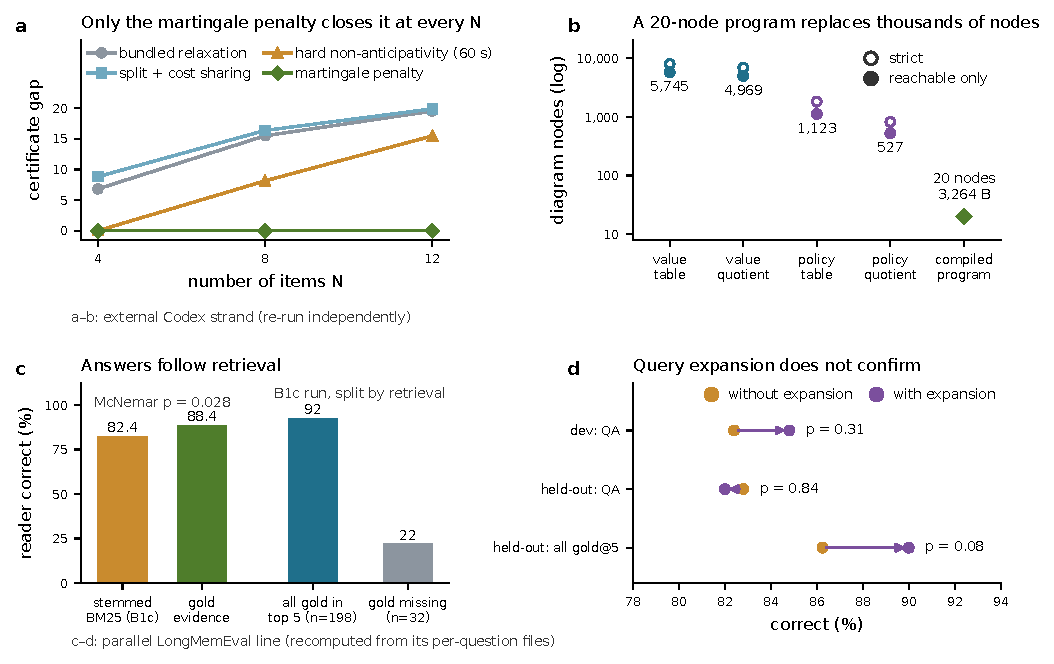
\includegraphics[width=\linewidth]{figures/fig6_external.pdf}
\caption{External strands. (a)~Certificate gap by relaxation family in the finite model. (b)~Size of the same $N=12$ optimum as value diagram, policy diagram and compiled program (log scale). (c)~Reader accuracy on LongMemEval by retrieval condition. (d)~Query expansion on development against held-out data.}
\label{fig:external}
\end{figure}

\section{Discussion}
Three things hold up. First, the programme's product claim did not survive a fair comparator: BM25 is better on every axis measured, and the code's cost is the fitted per-archive vocabulary, not the code. Second, two lossless compactions exist and are free to adopt. Third, and most transferable, verdicts in this domain are fragile to configuration choices that papers rarely state: the document unit, the averaged cohort, the arm family used for an ablation, the benchmark and the declared metric. A reader of a single number cannot tell which of these was fixed, and the same arms on the same data gave opposite verdicts when one of them changed.

Two practical rules follow. Every reported difference should name its document unit, cohort, comparator, scorer, metric and tie rule. In an audit of this programme's own reading layer, none of «p4.retrieval_units|0» retrieval claims named all five fields that were checked. Every gate should declare a minimum useful effect, not only significance. The one gate in this programme without it passed an arm that closed «policy.closed_bm25_pct|1»\% of the gap it was meant to close.

The only live lead is fusion with a small fixed weight. Its value is bounded by what the parallel line measured: answers follow retrieval, but the gap between the all-gold and the missing-gold conditions («par.qa2.allgold_pct|0»\% against «par.qa2.missing_pct|0»\%) means that each point of all@5 is worth at most about «expr:({par.qa2.allgold_pct}-{par.qa2.missing_pct})/100|1» points of answer accuracy. The two lines also use different document units (sessions there, turns here). A confirmation would need unseen data, a hash-committed protocol, and a comparison against stemmed BM25.

\section{Limitations and process disclosures}\label{sec:limits}
\begin{itemize}\setlength{\itemsep}{1pt}
\item \textbf{Not preregistered.} Gates were written into run records before results, but none was hash-committed in advance. For the channel ablation, the only evidence of ordering is file modification times.
\item \textbf{No independent audit of this programme's own code.} The implementer and the auditor were the same agent for everything except the review of the external strand.
\item \textbf{All data has been seen.} Both lines have now looked at every answerable LongMemEval-S question. The parallel line's split puts «par.split.discovery|0», «par.split.development|0» and «par.split.final_locked|0» questions in its discovery, development and locked sets. Of these, «par.split.overlap.discovery|0», «par.split.overlap.development|0» and «par.split.overlap.final_locked|0» are inside this programme's pilot set. No unseen test set remains on disk.
\item \textbf{Licences.} RealTalk has no published licence. LoCoMo and PerLTQA are non-commercial.
\item \textbf{Prototype costs.} Byte counts are reachable-object accounting. The comparators are Python prototypes, not production engines.
\item \textbf{Supersessions.} The programme's supersession ledger of 17 September records «sup.entries|0» entries, «expr:{sup.status.RETRACTED}+{sup.status.FULLY_RETRACTED}|0» of them retractions (Table~\ref{tab:supersession}). Its arithmetic reproduced; what broke was what numbers were compared against, what they were called and what was concluded from them.
\item \textbf{The head researcher's own errors.} They are listed in Table~\ref{tab:corrections}. They include a published REFUTED verdict that had to be withdrawn, an unqualified subgroup result and an estimate reported as if measured.
\end{itemize}

\begin{table}[tbp]
\centering
\footnotesize
\caption{The head researcher's own errors in this programme, all corrected in the record where they appeared.}
\label{tab:corrections}
\begin{tabularx}{\linewidth}{@{}l >{\raggedright\arraybackslash}p{5.2cm} >{\raggedright\arraybackslash}X@{}}
\toprule
Date & What was wrong & Correction \\
\midrule
2026-09-17 $\to$ 09-20 & Accumulation-order hypothesis recorded as REFUTED; withdrawn & 6 forced permutations against a 12.5\% event miss it with probability 0.45; the null was uninformative \\
2026-09-20 & Bigram-analyser explanation of the LoCoMo gap proposed and falsified & the project's frozen arm already used that analyser \\
2026-09-20 & Rare-bucket subgroup quoted as a LoCoMo-wide result & 48 B $-$ 12 B is +31.77 pp in the rare bucket (n = 950) but +19.67 on all 1{,}535 queries \\
2026-09-20 & Claim-screen denominator & 37 retrieval claims, not one more: a heading line had merged into a paragraph \\
2026-09-20 & Sign bug in the claim trace index & negative-valued claims looked untraceable; matching by absolute value fixed it \\
2026-09-21 & Resident memory described as dense float arrays & measured: character vocabulary 16.81 MB and word vocabulary 8.03 MB \\
2026-09-21 & LoCoMo channel result described as "neutral" & reworded: no significant difference was demonstrated, [\textminus{}2.05, 0.83] pp \\
2026-09-21 & RealTalk word-only lead from unprojected arms & reversed at $k=96$: \textminus{}2.69 pp \\
2026-09-22 & Codex role summary read as a count of distinct roles & it is the bitwise OR of role masks; the package was right \\
2026-09-22 & Policy-shaped gate written without a minimum effect & passed while closing 9.7\% of the gap to BM25 and 1.57\% of the gap to the floor \\
2026-09-23 & Compact BM25 size estimated, not measured & estimate 151 kB (5.3$\times$); measured 211{,}608 B (3.79$\times$) \\
\bottomrule
\end{tabularx}
\end{table}


\section{Data and code availability}
This paper, its claims ledger and the scripts that regenerate every figure, table and number from the ledger are public at \url{https://github.com/haliltalhaertan/llmzip-paper}. The code is released under the MIT licence; the text, figures, tables and ledger are released under CC BY 4.0. The programme's run records and code live in a private development repository. For every number, the ledger (\texttt{CLAIMS\_LEDGER.csv}) records the source file within that archive, the field read and the file's SHA-256. \texttt{build\_ledger.py} documents each extraction but needs the private archive to run. Benchmark text is not redistributed. The two external strands of Section~\ref{sec:external} are summarised only; their packages are not included.

\bibliographystyle{plainnat}
\bibliography{references}

\FloatBarrier
\clearpage
\appendix
\section{Complete result tables}
\begin{table}[H]
\centering
\footnotesize
\caption{C1 gate, all twelve cells (RealTalk, pp, 95\% intervals).}
\label{tab:c1}
\begin{adjustbox}{max width=\linewidth}\begin{tabular}{@{}l r l l l l@{}}
\toprule
& & \multicolumn{2}{c}{vs BM25, coarse analyser} & \multicolumn{2}{c}{vs BM25, production analyser} \\
\cmidrule(lr){3-4}\cmidrule(l){5-6}
Arm & B/doc & $\Delta$FR@3 & $\Delta$Hit@10 & $\Delta$FR@3 & $\Delta$Hit@10 \\
\midrule
\texttt{k96/sym} & 12 & \textminus{}11.04 [\textminus{}15.71, \textminus{}7.09] & \textminus{}8.79 [\textminus{}13.50, \textminus{}4.68] & \textminus{}13.18 [\textminus{}17.75, \textminus{}9.19] & \textminus{}15.18 [\textminus{}18.82, \textminus{}11.74] \\
\texttt{k96/qscale} & 12 & \textminus{}11.49 [\textminus{}16.52, \textminus{}7.05] & \textminus{}5.67 [\textminus{}12.15, 0.00] & \textminus{}13.64 [\textminus{}18.64, \textminus{}9.06] & \textminus{}12.06 [\textminus{}17.55, \textminus{}6.70] \\
\texttt{k192/sym} & 24 & \textminus{}5.34 [\textminus{}7.20, \textminus{}3.66] & \textminus{}3.55 [\textminus{}7.74, 1.14] & \textminus{}7.49 [\textminus{}9.27, \textminus{}6.08] & \textminus{}9.93 [\textminus{}12.62, \textminus{}7.26] \\
\texttt{k192/qscale} & 24 & \textminus{}4.15 [\textminus{}6.18, \textminus{}2.21] & +0.00 [\textminus{}4.90, 5.17] & \textminus{}6.29 [\textminus{}8.67, \textminus{}4.09] & \textminus{}6.38 [\textminus{}9.94, \textminus{}2.26] \\
\texttt{k384/sym} & 48 & \textminus{}2.42 [\textminus{}4.27, \textminus{}0.83] & \textminus{}1.14 [\textminus{}5.51, 3.13] & \textminus{}4.57 [\textminus{}6.84, \textminus{}2.16] & \textminus{}7.52 [\textminus{}10.85, \textminus{}4.29] \\
\texttt{k384/qscale} & 48 & \textminus{}1.11 [\textminus{}2.26, 0.05] & +2.55 [\textminus{}0.14, 5.50] & \textminus{}3.26 [\textminus{}5.80, \textminus{}0.95] & \textminus{}3.83 [\textminus{}5.74, \textminus{}2.10] \\
\bottomrule
\end{tabular}\end{adjustbox}
\end{table}

\begin{table}[H]
\centering
\footnotesize
\caption{LoCoMo contrasts under both document units and both cohorts (95\% intervals).}
\label{tab:n2}
\begin{adjustbox}{max width=\linewidth}\begin{tabular}{@{}l l l l l@{}}
\toprule
& \multicolumn{2}{c}{Project unit} & \multicolumn{2}{c}{External unit} \\
\cmidrule(lr){2-3}\cmidrule(l){4-5}
Contrast (FR@3, pp) & rare bucket & all queries & rare bucket & all queries \\
\midrule
48 B $-$ 12 B sign & +31.77 [27.58, 35.95] & +19.67 [16.65, 22.90] & +21.03 [18.27, 24.00] & +12.14 [9.76, 14.52] \\
48 B sign $-$ BM25 & +1.58 [\textminus{}0.73, 3.88] & +1.31 [\textminus{}0.34, 3.05] & \textminus{}1.80 [\textminus{}4.14, 0.57] & \textminus{}0.60 [\textminus{}2.07, 0.78] \\
full sign $-$ BM25 & \textminus{}3.77 [\textminus{}6.51, \textminus{}0.63] & \textminus{}1.75 [\textminus{}3.61, 0.68] & \textminus{}6.08 [\textminus{}8.46, \textminus{}3.71] & \textminus{}3.57 [\textminus{}5.14, \textminus{}1.98] \\
48 B standardized $-$ BM25 & +3.02 [0.27, 5.64] & +2.64 [0.81, 4.49] & +1.64 [\textminus{}0.59, 3.89] & +1.76 [0.37, 3.26] \\
full raw float $-$ BM25 & \textminus{}19.81 [\textminus{}24.20, \textminus{}15.52] & \textminus{}12.36 [\textminus{}15.47, \textminus{}9.50] & \textminus{}2.18 [\textminus{}6.76, 1.75] & \textminus{}0.17 [\textminus{}2.90, 2.45] \\
\bottomrule
\end{tabular}\end{adjustbox}
\end{table}

\begin{table}[H]
\centering
\footnotesize
\caption{Channel ablation at $k=96$ with sign codes (pp, 95\% intervals).}
\label{tab:channels}
\begin{adjustbox}{max width=\linewidth}\begin{tabular}{@{}l r l l r@{}}
\toprule
Benchmark & all channels FR@3 & word only $-$ all & word+LSA $-$ all & memory saved by word only (\%) \\
\midrule
LongMemEval & 54.60 & \textminus{}3.84 [\textminus{}6.88, \textminus{}0.75] & \textminus{}4.40 [\textminus{}7.48, \textminus{}1.28] & 60 \\
RealTalk & 22.87 & \textminus{}2.69 [\textminus{}4.45, \textminus{}0.66] & \textminus{}2.18 [\textminus{}4.25, \textminus{}0.38] & 69 \\
LoCoMo & 23.70 & \textminus{}0.52 [\textminus{}2.05, 0.83] & \textminus{}1.49 [\textminus{}3.06, 0.41] & 68 \\
PerLTQA & 49.09 & +2.40 [1.14, 3.67] & +3.13 [1.96, 4.26] & 69 \\
\bottomrule
\end{tabular}\end{adjustbox}
\end{table}

\begin{table}[H]
\centering
\footnotesize
\caption{RealTalk ladder, all seventeen arms (\%). NOPROJ arms are unprojected and not compact.}
\label{tab:ladder}
\begin{adjustbox}{max width=\linewidth}\begin{tabular}{@{}l r r@{}}
\toprule
Arm & Hit@10 & FR@3 \\
\midrule
\texttt{BM25\_frozen/-} & 61.70 & 36.05 \\
\texttt{BM25\_coarse/-} & 55.32 & 33.91 \\
\texttt{NOPROJ\_FULL/float} & 47.80 & 28.07 \\
\texttt{NOPROJ\_FULL/qscale} & 63.97 & 38.62 \\
\texttt{NOPROJ\_FULL/sym} & 7.94 & 4.90 \\
\texttt{NOPROJ\_WORD/float} & 56.03 & 31.19 \\
\texttt{NOPROJ\_WORD/qscale} & 59.57 & 35.73 \\
\texttt{NOPROJ\_WORD/sym} & 2.84 & 1.46 \\
\texttt{k192/float} & 40.43 & 19.74 \\
\texttt{k192/qscale} & 55.32 & 29.75 \\
\texttt{k192/sym} & 51.77 & 28.56 \\
\texttt{k384/float} & 43.69 & 24.30 \\
\texttt{k384/qscale} & 57.87 & 32.79 \\
\texttt{k384/sym} & 54.18 & 31.48 \\
\texttt{k96/float} & 36.60 & 17.25 \\
\texttt{k96/qscale} & 49.65 & 22.41 \\
\texttt{k96/sym} & 46.52 & 22.87 \\
\bottomrule
\end{tabular}\end{adjustbox}
\end{table}

\begin{table}[H]
\centering
\footnotesize
\caption{The programme's supersession ledger of 2026-09-17: 20 entries, of which 8 are retractions.}
\label{tab:supersession}
\begin{tabularx}{\linewidth}{@{}l >{\raggedright\arraybackslash}X l >{\raggedright\arraybackslash}X@{}}
\toprule
Entry & Status & Entry & Status \\
\midrule
\texttt{ASYM-TWO-DEFINITIONS} & closed for rank based metrics & \texttt{GATE-C1-IMPLEMENTATION} & defective \\
\texttt{BM25-RAW-TEXT} & corrected & \texttt{GATE-C1-THIRD-DEFECT} & retracted \\
\texttt{BRIEF3-C1b} & retracted & \texttt{NOVELTY-GENUINELY-OURS} & not verified \\
\texttt{BRIEF3-C1c} & survives & \texttt{PERLTQA-HIGHK-MECHANISM} & open \\
\texttt{BRIEF3-C2} & fully retracted & \texttt{RANK-OVERFLOW} & retracted \\
\texttt{BRIEF3-C6b} & retracted & \texttt{RERANK-DISSOLUTION} & narrowed \\
\texttt{BRIEF3-W5} & fully retracted & \texttt{SIGMA-ONLY} & retracted \\
\texttt{EXPECTED-HIT-10} & data defect & \texttt{SIGN-BEATS-FLOAT-10PP} & corrected \\
\texttt{FINAL-STATE-AUTHORITY} & historical / non-authoritative & \texttt{STOP-SCOPE} & scope correction \\
\texttt{FLOAT96-UNCENTERED} & terminology correction & \texttt{TOKENIZER-OFFSET-TRANSPORT} & retracted \\
\bottomrule
\end{tabularx}
\end{table}


\end{document}
